\documentclass[a4paper,12pt]{report}
\usepackage[utf8]{inputenc}           % vagy latin2 helyett utf8
\usepackage[T1]{fontenc}              % karakterkódolás
\usepackage[hungarian]{babel}           % angol, magyar beállítások

%\usepackage[nottoc]{tocbibind}
%\usepackage{url}
\usepackage[hidelinks]{hyperref}
\hypersetup{
colorlinks=true,
linkcolor=black,
urlcolor=blue,
}
\urlstyle{same}

\usepackage{subcaption}
\usepackage{csquotes}
\usepackage{float}

%\bibliographystyle{plain}

\usepackage{listings}                 % forráskód-beágyazás

\usepackage{multicol}
\usepackage{longtable}

\frenchspacing                % helyközök
%\usepackage{times}           % betűtípus
\usepackage{lmodern}          % vagy inkább ez

\usepackage[margin=2.5cm,left=3.5cm,includeheadfoot]{geometry}
                              % margók
\usepackage{graphicx}         % képekhez
\usepackage{setspace}         % sorköz
\onehalfspacing               % másfeles

\usepackage{pgfplots}
\pgfplotsset{width=7cm,compat=1.12}


\begin{document}

% ------------------------------------------------------------------------------
% Címlap


\begin{titlepage}

\noindent
\parbox[m]{0.2\textwidth}{
%\includegraphics[width=0.2\textwidth]{elte_cimer_ff.eps}     % fekete-fehér
 
\includegraphics[width=0.2\textwidth]{elte_cimer_szines.eps} % színes
}
\hfill
\parbox[m]{0.7\textwidth}{
\begin{center}
\begin{large}
\textsc{
Eötvös Loránd Tudományegyetem\\
\vspace{0.5pc}
Informatikai Kar\\
\vspace{0.5pc}
Média- és Oktatásinformatikai tanszék\\
}
\end{large}
\end{center}
}

\vspace{1pc}
\hrule

\vfill

\begin{center}
{\LARGE Egy a mindennapokat megkönnyítő valós idejű okos otthon alkalmazás megvalósítása}
\end{center}

\vfill

\noindent
\hspace*{0.05\textwidth}
\parbox{0.45\textwidth}{
{\it Témavezető:}
\bigskip

{\Large Heizlerné Bakonyi Viktória }
\smallskip

Műszaki tanár
}
\hfill
\parbox{0.45\textwidth}{
{\it Szerző:}
\bigskip

{\Large Hegedüs Ádám}
\smallskip

Programtervező Informatikus BSc
}


\vfill

\begin{center}
{\large {\it Budapest, 2018}}
\end{center}

\end{titlepage}


% ------------------------------------------------------------------------------
% Témabejelentő

%\vspace*{\fill}
%\begin{center}
%Ehelyett az oldal helyett a Szakdolgozat-téma bejelentő szerepel.
%\end{center}
%\vfill
%\thispagestyle{empty}
%\newpage
\setcounter{page}{1}

% ------------------------------------------------------------------------------
% Tartalomjegyzék

\tableofcontents

% ------------------------------------------------------------------------------


\chapter{Bevezetés}

\section{Motiváció}
    Napjainkban mindent átsző a technnológia. Jelen van az oktatásban, egészségügyben, tömegközelekedésben, az élet rengeteg
    területén, de ami talán a legfontosabb, az otthonunkban. A legtöbb háztartásban előfordulnak okos eszközök, a család
    minden tagja ismerkedik a számítógép használatával, unokától kezdve a nagymamáig. De mégis mi célt szolgál a technológia?
    Szórakozás, információszerzés, kapcsolattartás távoli ismerősökkel, millió oka lehet annak hogy valaki laptopot ragadjon.
    Talán az egyik legfontosabb ezek közül az, hogy eszközeink segítsék, könnyebbé tegyék mindennapjainkat. Ez a gondolat
    motivált a dolgozatom megírására, szerettem volna egy olyan alkalmazást elkészíteni mely egyszerű funkciót tölbe, mégis
    hasznos lehet a dolgos hétköznapjainkon. Bárkivel előfordulhat hogy felkapcsolva felejti a lámpát a reggeli rohanás során
    és csak a munkahelyén jut eszébe. A szakdolgozatom erre a problémára szeretne megoldást kínálni. Az alkalmazás segítségével
    bárki regisztrálhat egy lámpát, akár több ember ugyanazt a fényforrást, és távolról fel -és lekapcsolhatja, követheti hogy
    mikor történt változás, illetve mennyi ideig volt összesen bekapcsolt állapotban az eszköz. Mindez valós időben történik,
    tehát minden felhasználó a legfrissebb információkkal rendelkezik a program használata közben.

\section{A programról}
    Az alkalmazás három részből áll, két kliensalkalmazásból, valamint egy szerverből. A Windows 10 klienst használhatják
    bejelentkezett felhasználók, ezen a kényelmes felületen találhatják a fő funckiókat, lámpát adhatnak hozzá profiljukhoz, valós időben
    vezérelhetik azt, megtekinthetik az eszköz statisztikáit. A másik kliensalkalmazást egy Raspberry Pi 3 mikroprocesszor futtatja, mely
    rá van kötve a vezérelni kívánt lámpára, szabályozza annak áramellátását, a szervertől kapott utasítások alapján. Minden változás után
    visszaigazolja a sikeres kapcsolást, valamint módosítások körülményeit is elküldi a szervernek, így az rögzítheti az eseményeket az
    adatbázisban. A szerver tehát köztes szerepet tölt be, a felhasználó rajta keresztül tud üzenni a eszközének, a lámpa pedig tőle
    kapja az utasításokat. Az adatbázis-kezelés is az ő feladata.

\begin{figure}[h!]
    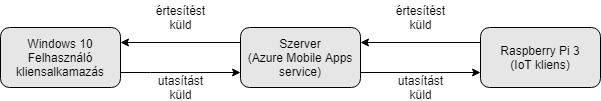
\includegraphics[width=\linewidth]{images/application_diagram.jpg}
    \caption{Az alkalmazás struktúrája}
    \label{fig: Az alkalmazás struktúrája}
\end{figure}

\chapter{Felhasználói dokumentáció}

\section{Minimális rendszerkövetelmények}
    A felhasználónak az alábbiakra van szüksége a program használatához:

    \begin{itemize}
        \item Egy Raspberry Pi 3 Model B mikroprocesszor, Windows 10 IoT Core operációs rendszerrel
        \item Windows 10 asztali vagy mobil eszköz
        \item Facebook profil
    \end{itemize}

\section{Raspberry Pi}

\subsection{Az eszközről}
    A Raspberry Pi egy bankkártya méretű, egyetlen áramköri lapra integrált számítógép, melyet az Egyesült Királyságban
    helyeztek forgalmomba 2012-ben, főleg oktatási célokra. Azóta számos változata megjelent, a szakdolgozat elkészítéséhez
    egy Raspberry Pi 3 Model B-t használtam. Számos bemenettel rendelkezik, többek között Ethernet csatlakozóval, HDMI, USB
    portokkal, a felhasznált modell pedig már beépített Wi-Fi adapterrel is. Többféle operációs rendszert telepíthetünk rá,
    köztük a Windows 10 IoT Core-t is, így kiválóan alkalmas arra, hogy futtathassuk rajta az IoT kliensalkalmazást. A továbbiakban
    a mikroprocesszor konfigurálása következik.

\begin{figure}[h!]
    \hspace{5cm}
    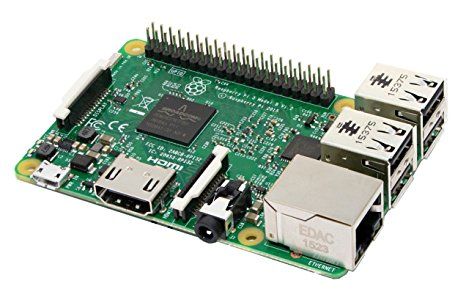
\includegraphics[width=6cm]{images/raspberry_pi3.jpg}
    \caption{Raspberry Pi 3 Model B}
    \label{fig: Raspberry Pi 3}
\end{figure}

\subsection{Beszerzés}
    A program futtatásához az eszköz korábbi verziói is megfelelőek lehetnek, azonban érdemes lehet a fent említett Raspberry Pi 3
    Model B -t, illetve az ennél újabb kiadásokat beszerezni, mivel ezek bizonyítottan elég erős hardverrel és csatlakozókkal rendelkeznek
    a feladat ellátásához. A szükséges komponensek:

\begin{itemize}
    \item Raspberry Pi 3 model B 1GB RAM Quad Core 2016-os alaplap
    \item 1.2A-es Sunny tápegység, 24 órás üzemre tervezve
    \item Legalább 8GB tárolókapacitású microSD kártya
\end{itemize}

    Az eszközt magyar viszonteladóktól is be lehet szerezni, valamint lehetőség van különböző előre összeállított csomagokat megvásárolni,
     melyek a fent említett kötelező elemeken túl tartalmazhatnak védőtokot az alaplapnak, illetve előtelepített operációs rendszert.

    A dolgozathoz használt kiszerelés az alábbi \href{https://malnapc.hu/yis/raspberry-pi-3-quad-core-suli-kit}{linken} elérhető.

\subsection{Operációs rendszer telepítése Raspberry Pi eszközre}

\subsubsection{Telepítés előtelepített SD kártyáról}
    Ha olyan verziót vásároltunk, melyhez előtepített operációs rendszert járt, akkor nincs más dolgunk, helyezzük be az SD kártyát
    az alaplapba, kössük össze a tápegységgel, helyezzük áram alá, s az eszköz azonnal elindul. Egy HDMI kábel segítségével kössük össze
    monitorunkkal, a vezérléshez szükség lesz legalább egy egérre. Az internetelérés történhet Ethernet csatlakozón, vagy (legalább Raspberry
    Pi 3 esetén) Wi-Fi-n keresztül is. Ha mindent jól csináltunk, akkor az eszköz rövid betöltés után megjelenít egy ablakot,
    melyben kiválaszthatjuk az általunk kívánt operációs rendszert. Többet is telepíthetünk, és javasolt is az alapértelmezett Raspbiant,
    valamint számunkra létfontosságú Windows 10 IoT Core-t. Ezt a Raspberry le fogja tölteni, ezért \textbf{elengedhetetlen} az internetkapcsolat.
    Az eszköz automatikusan telepíti a kiválasztott rendszereket, miután végzett, a mikroprocesszorunk használatra alkalmas.

\begin{figure}[h!]
    \hspace{5cm}
    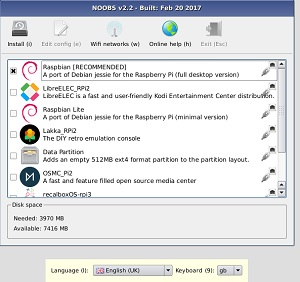
\includegraphics[width=6cm]{images/rpi_os_setup.jpg}
    \caption{Raspberry Pi Operációs rendszer kiválasztása}
    \label{fig: Raspberry Pi Operációs rendszer}
\end{figure}

\subsubsection{Telepítés nem előtelepített SD kártyáról}
    Ha nincs előre telepítve a szükséges operációs rendszer, akkor nekünk kell letölteni hivatalos forrásból.
    Ehhez a microsoft készített egy könnyen kezelhető felületet, a Windows 10 IoT Core Dashboardot, melyet
    \href{https://developer.microsoft.com/en-us/windows/iot/Downloads.htm}{ide} kattintva tudunk letölteni.
    Telepítsük fel az alkalmazást, majd kattintsunk a "\textbf{Set up a new device}" fülre, töltsük ki a szükséges adatokat, helyezzük
    az SD kártyát a számítógépünkbe. A "\textbf{Download and install}" lehetőségre klikkelve az alkalmazás telepíti nekünk
    az operációs rendszert.
    Ezt követően a lépések megegyeznek az előtelepítéses utasításokkal, tegyük a microSD-t a mikroprocesszorunkba, csatlakoztassuk
    a tápegységet, szükséges perifériákat, a rendszer rövid időn belül betölt.

    A részletes leírás az alábbi linken tekinthető meg: \url{https://www.windowscentral.com/how-install-windows-10-iot-raspberry-pi-3}

\subsection{Lámpa csatlakoztatása Raspberry Pi eszközhöz}
    Mivel nem rendelkezem mérnöki háttérismeretekkel, ezért nem egy valódi lámpát, hanem egy LED-et használtam a szakdolgozatom
    elkészítése során, így a LED működtetéséhez szükséges lépéseket, eszközöket fogom ismertetni.

\subsubsection{Szükséges elemek}

\begin{enumerate}
    \item \textbf{Egy} tetszőleges színű LED 2 - 2.5V-os fényforrás
    \item \textbf{Egy} próbapanel
    \item \textbf{Egy} legalább 270 Ohm-os ellenállás, a szakdolgozathoz 470 Ohm-ost használtam
    \item \textbf{Két} darab ANYA-APA Jumper kábel
\end{enumerate}

\begin{figure}[h!]
    \centering
    \begin{subfigure}[b]{0.4\linewidth}
        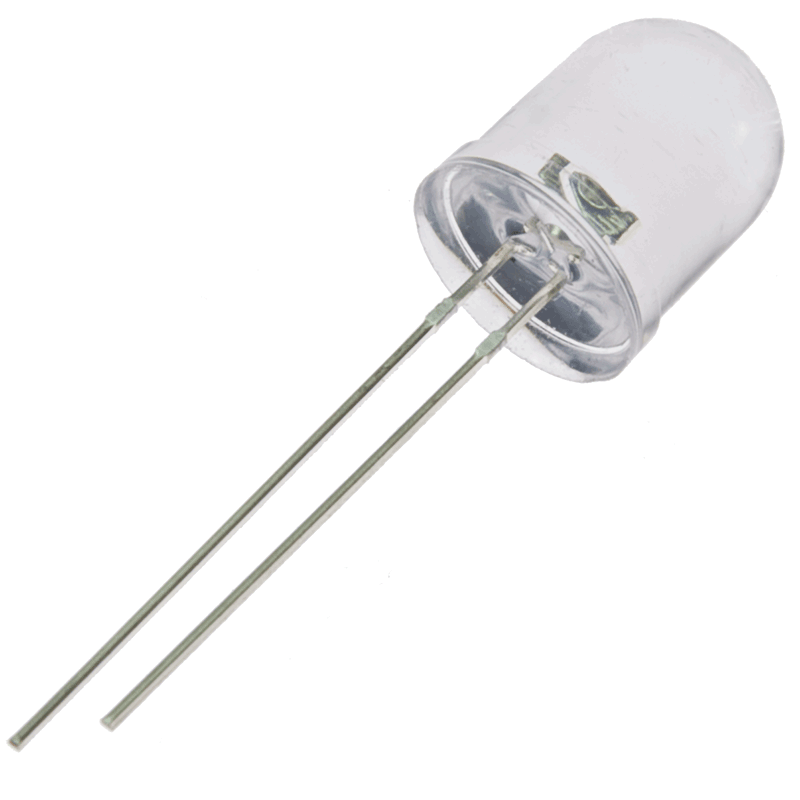
\includegraphics[width=\linewidth]{images/led.png}
        \caption{LED}
    \end{subfigure}
    \begin{subfigure}[b]{0.4\linewidth}
        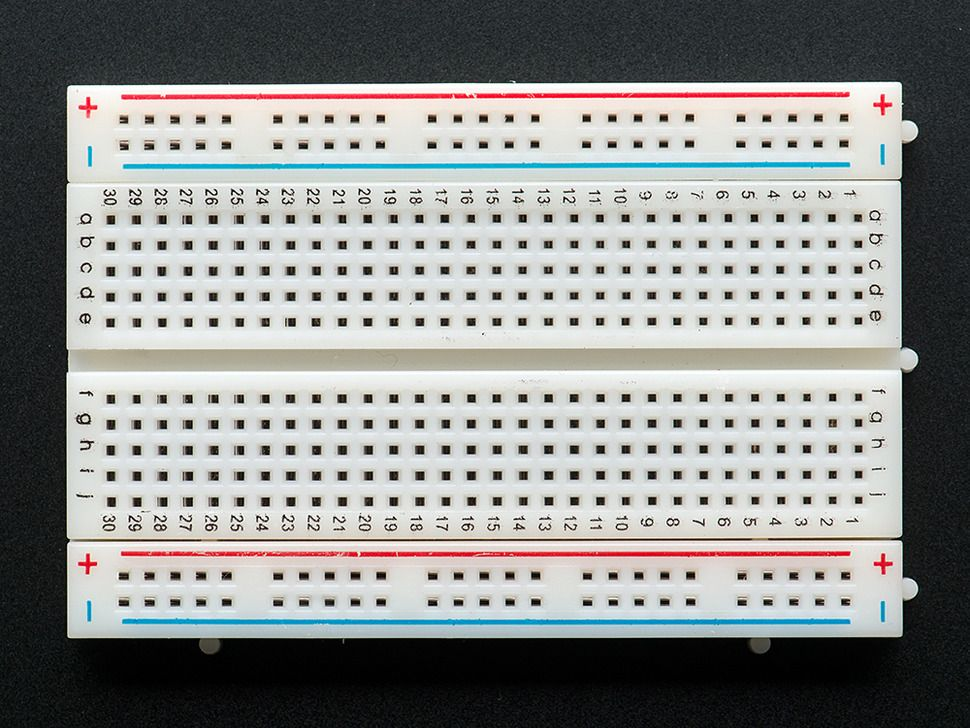
\includegraphics[width=\linewidth]{images/probapanel.jpg}
        \caption{Próbapanel}
    \end{subfigure}
    \begin{subfigure}[b]{0.4\linewidth}
        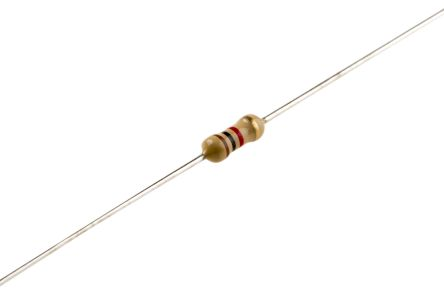
\includegraphics[width=\linewidth]{images/ellenallas.jpg}
        \caption{Ellenállás}
    \end{subfigure}
    \begin{subfigure}[b]{0.4\linewidth}
        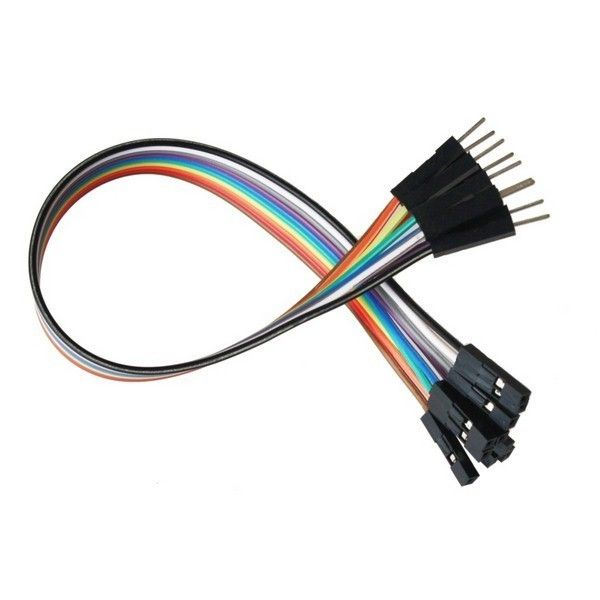
\includegraphics[width=\linewidth]{images/anyaapa.jpg}
        \caption{ANYA-APA kábel}
    \end{subfigure}
    \caption{Szükséges elemek}
    \label{fig:lampaelemek}
\end{figure}

\subsubsection{Összeszerelés}
    Miután beszereztük a szükséges elemeket, megkezdhetjük az összeszerelést. A próbapanelbe fogjuk belehelyezni a LED-et,
    az ellenállást, és a jumper kábel megfelelő végét. A másik végét a Raspberry Pi megfelelő GPIO pinjeire fogjuk csatlakoztatni.
    Ahhoz hogy a pinek között tudjunk tájékozódni, érdemes vásárolni egy kártyát, melyet rá lehet szúrni a tüskékre, és lehet látni
    a számozást.

\begin{figure}[h!]
    \hspace{5cm}
    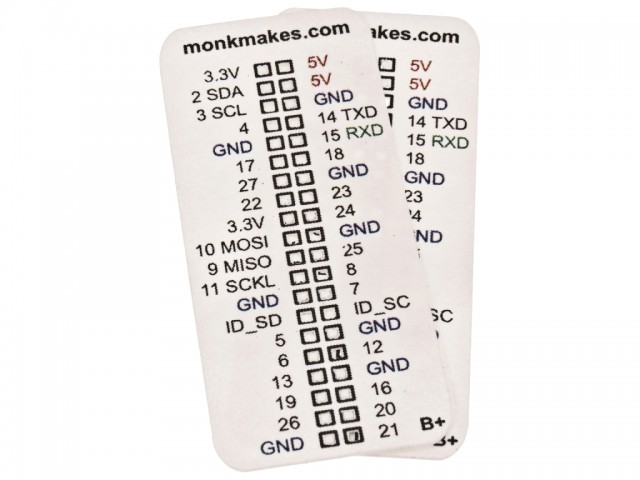
\includegraphics[width=6cm]{images/gpiohelper.jpg}
    \caption{A GPIO pinekhez kapható segítség}
    \label{fig: Pin segítség}
\end{figure}

    Készítsük magunk elé a mikroprocesszort és a többi szükséges eszközt, majd kövessük a következő lépéseket:

\begin{enumerate}
    \item A LED \textbf{hosszabbik} lábát szúrjuk bele a próbapanel \textbf{E} oszlopának \textbf{6.} sorába
    \item A LED \textbf{rövidebb} lába kerüljön egyel a hosszabbik alá, tehát a \textbf{E} oszlop \textbf{7.} sorába
    \item Hajlítsuk meg az ellenállás lábait úgy, hogy egy \textbf{U} alakot formáljon
    \item Egyik lábát helyezzük a LED hosszabbik vége mellé, tehát a \textbf{D 7} mezőbe
    \item A másik végződést szúrjuk a \textbf{D 1} helyre
    \item Fogjunk két ANYA-APA kábelt, az egyik APA végét szúrjuk az \textbf{A 1}, a másikét az \textbf{A 7} helyre, a LED
    rövidebb lábával egy sorba.
    \item Az első kábel ANYA végét csatlakoztassuk a Raspberry Pi 3.3V-os kimenetelére. Ez a bal felső kimenet a mikroprocesszoron.
    \item Végezetül a második kábel szabad végét kössük a 4-es GPIO pin-re. Ehhez használjuk a kis kártyát ha nem vagyunk biztosak
    magunkban.
\end{enumerate}

\begin{figure}[h!]
    \centering
    \begin{subfigure}[b]{0.4\linewidth}
        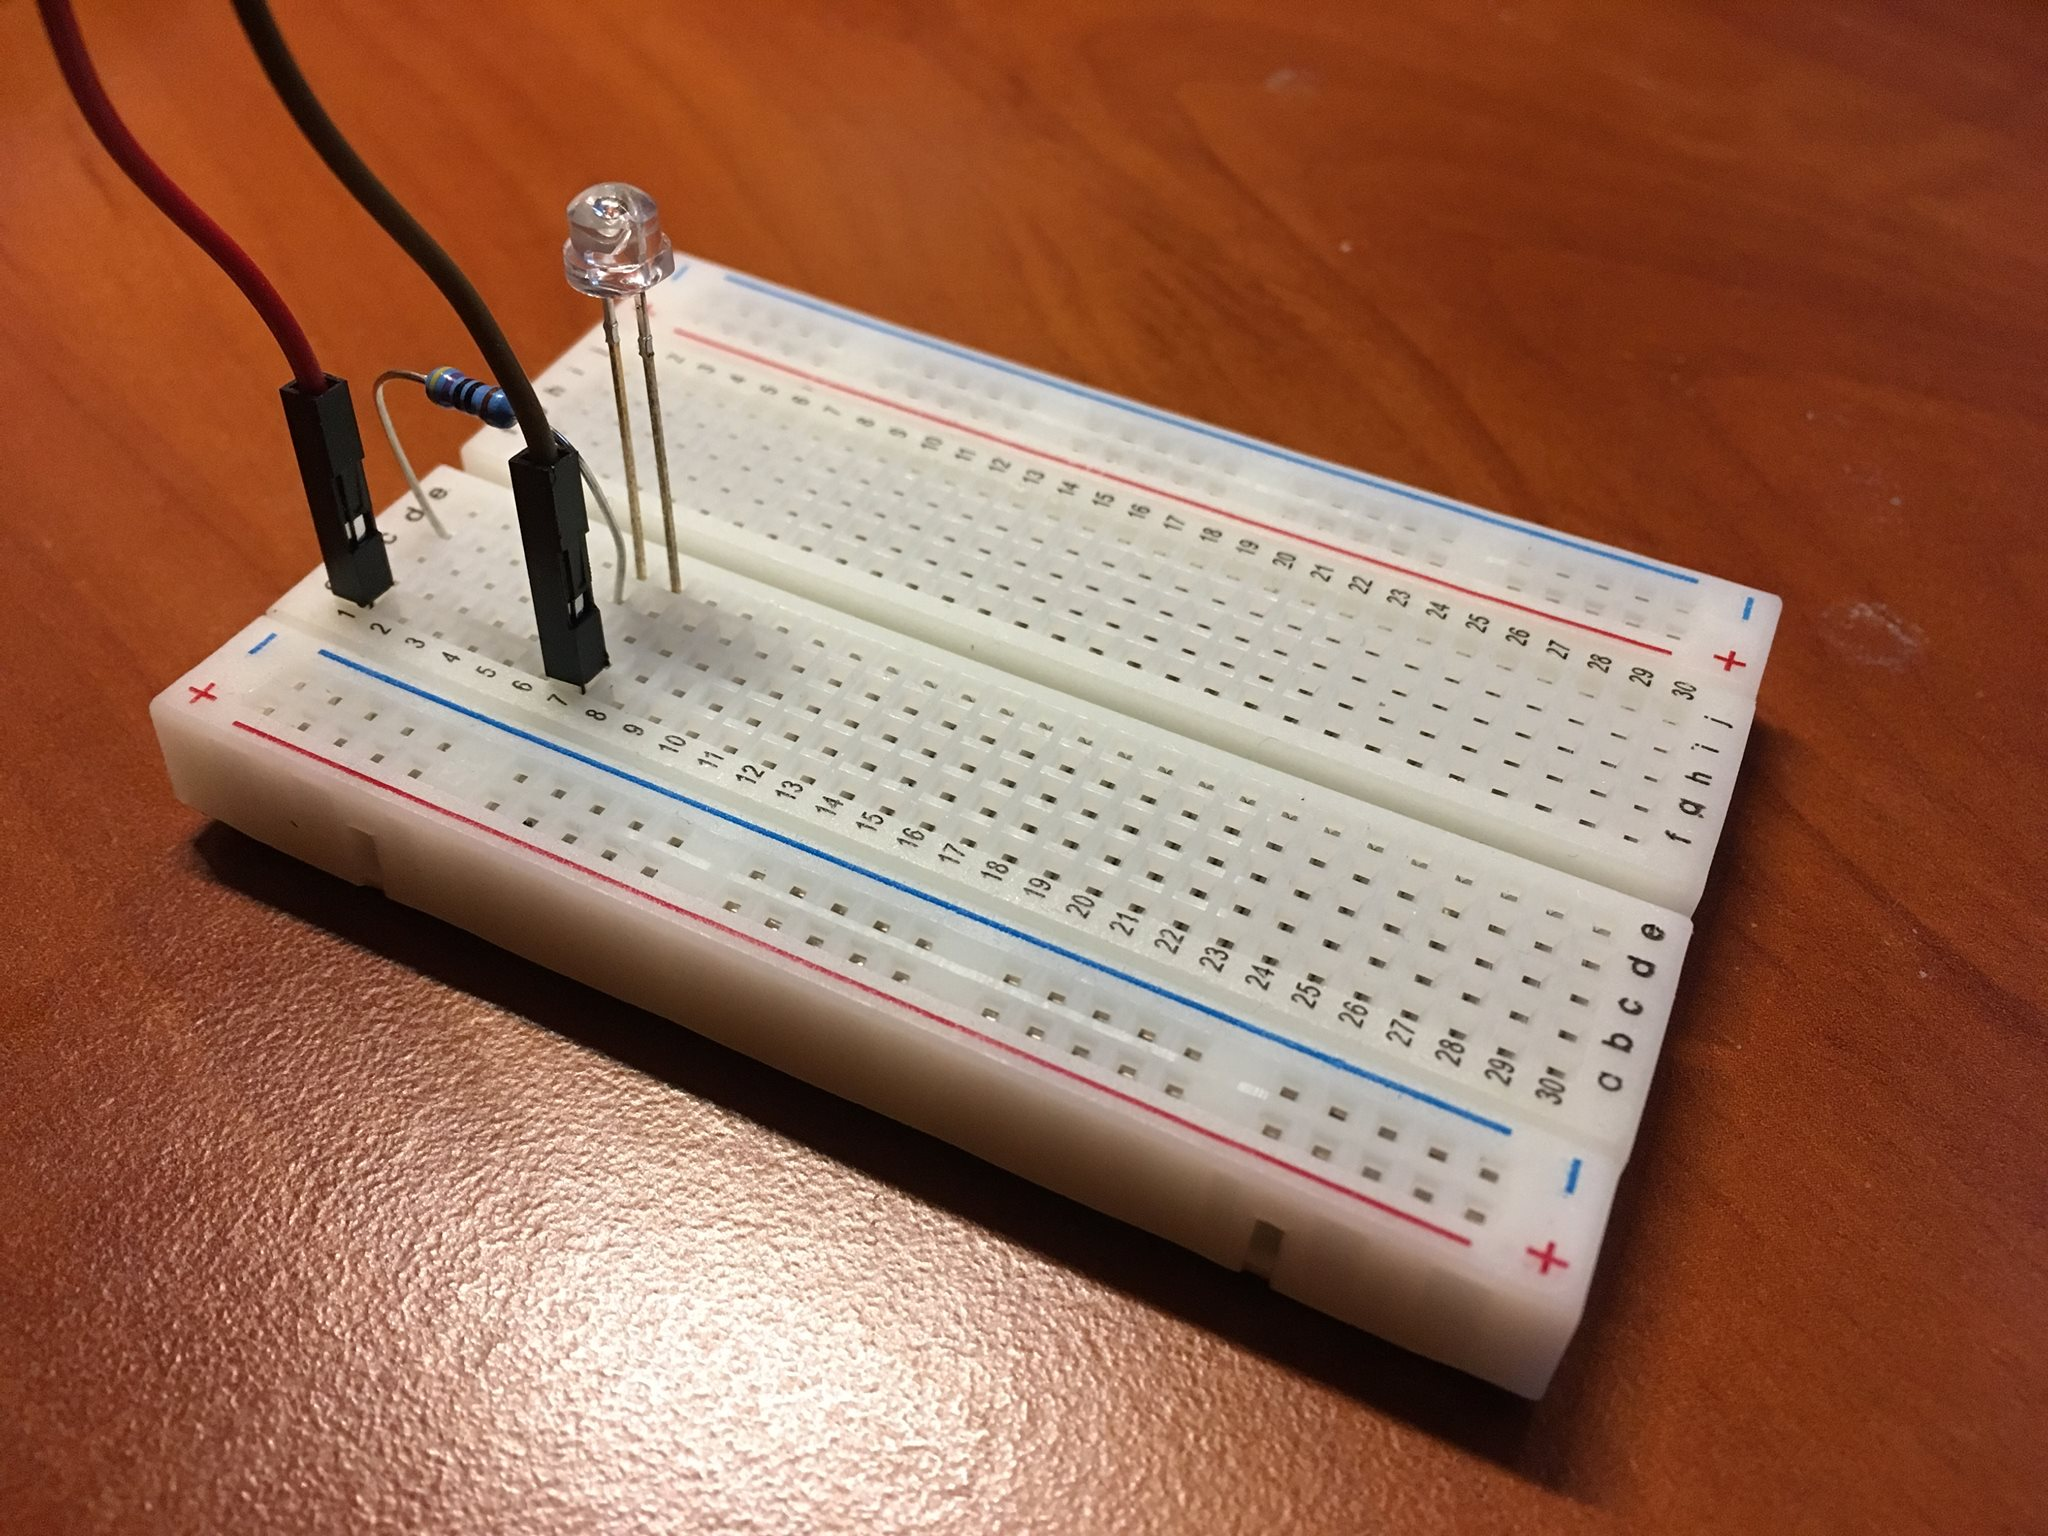
\includegraphics[width=\linewidth]{images/osszeszerelt1.jpg}
        \caption{Összeszerelt próbapanel oldalról}
    \end{subfigure}
    \begin{subfigure}[b]{0.4\linewidth}
        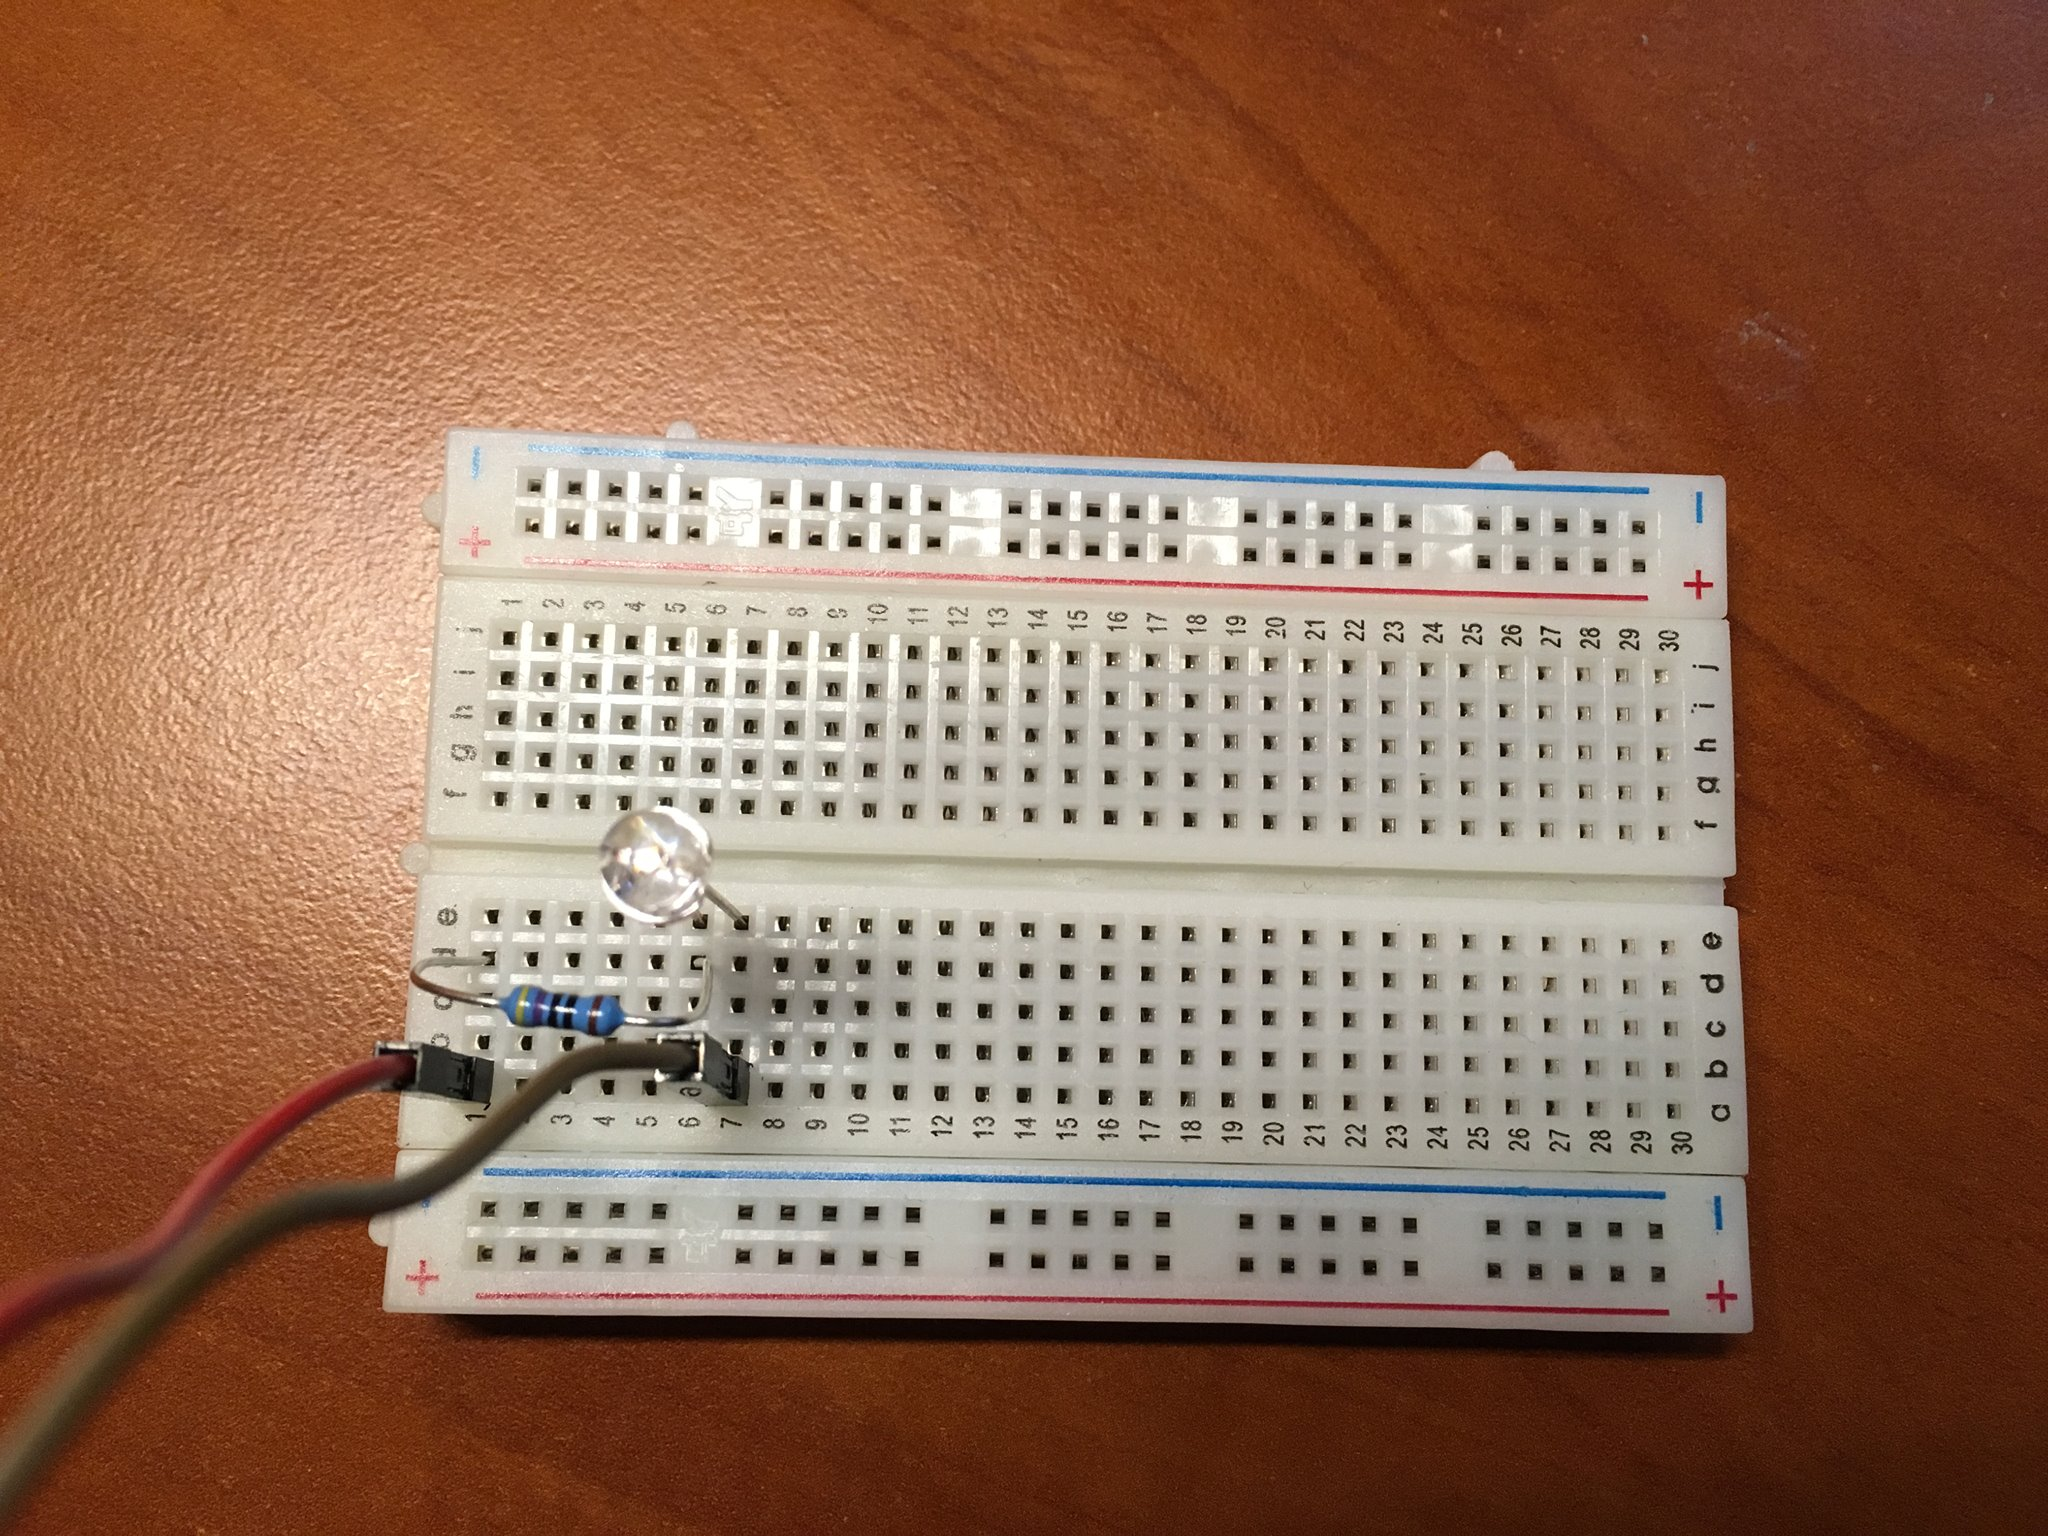
\includegraphics[width=\linewidth]{images/osszeszerelt2.jpg}
        \caption{Összeszerelt próbapanel felülről}
    \end{subfigure}
    \begin{subfigure}[b]{0.5\linewidth}
        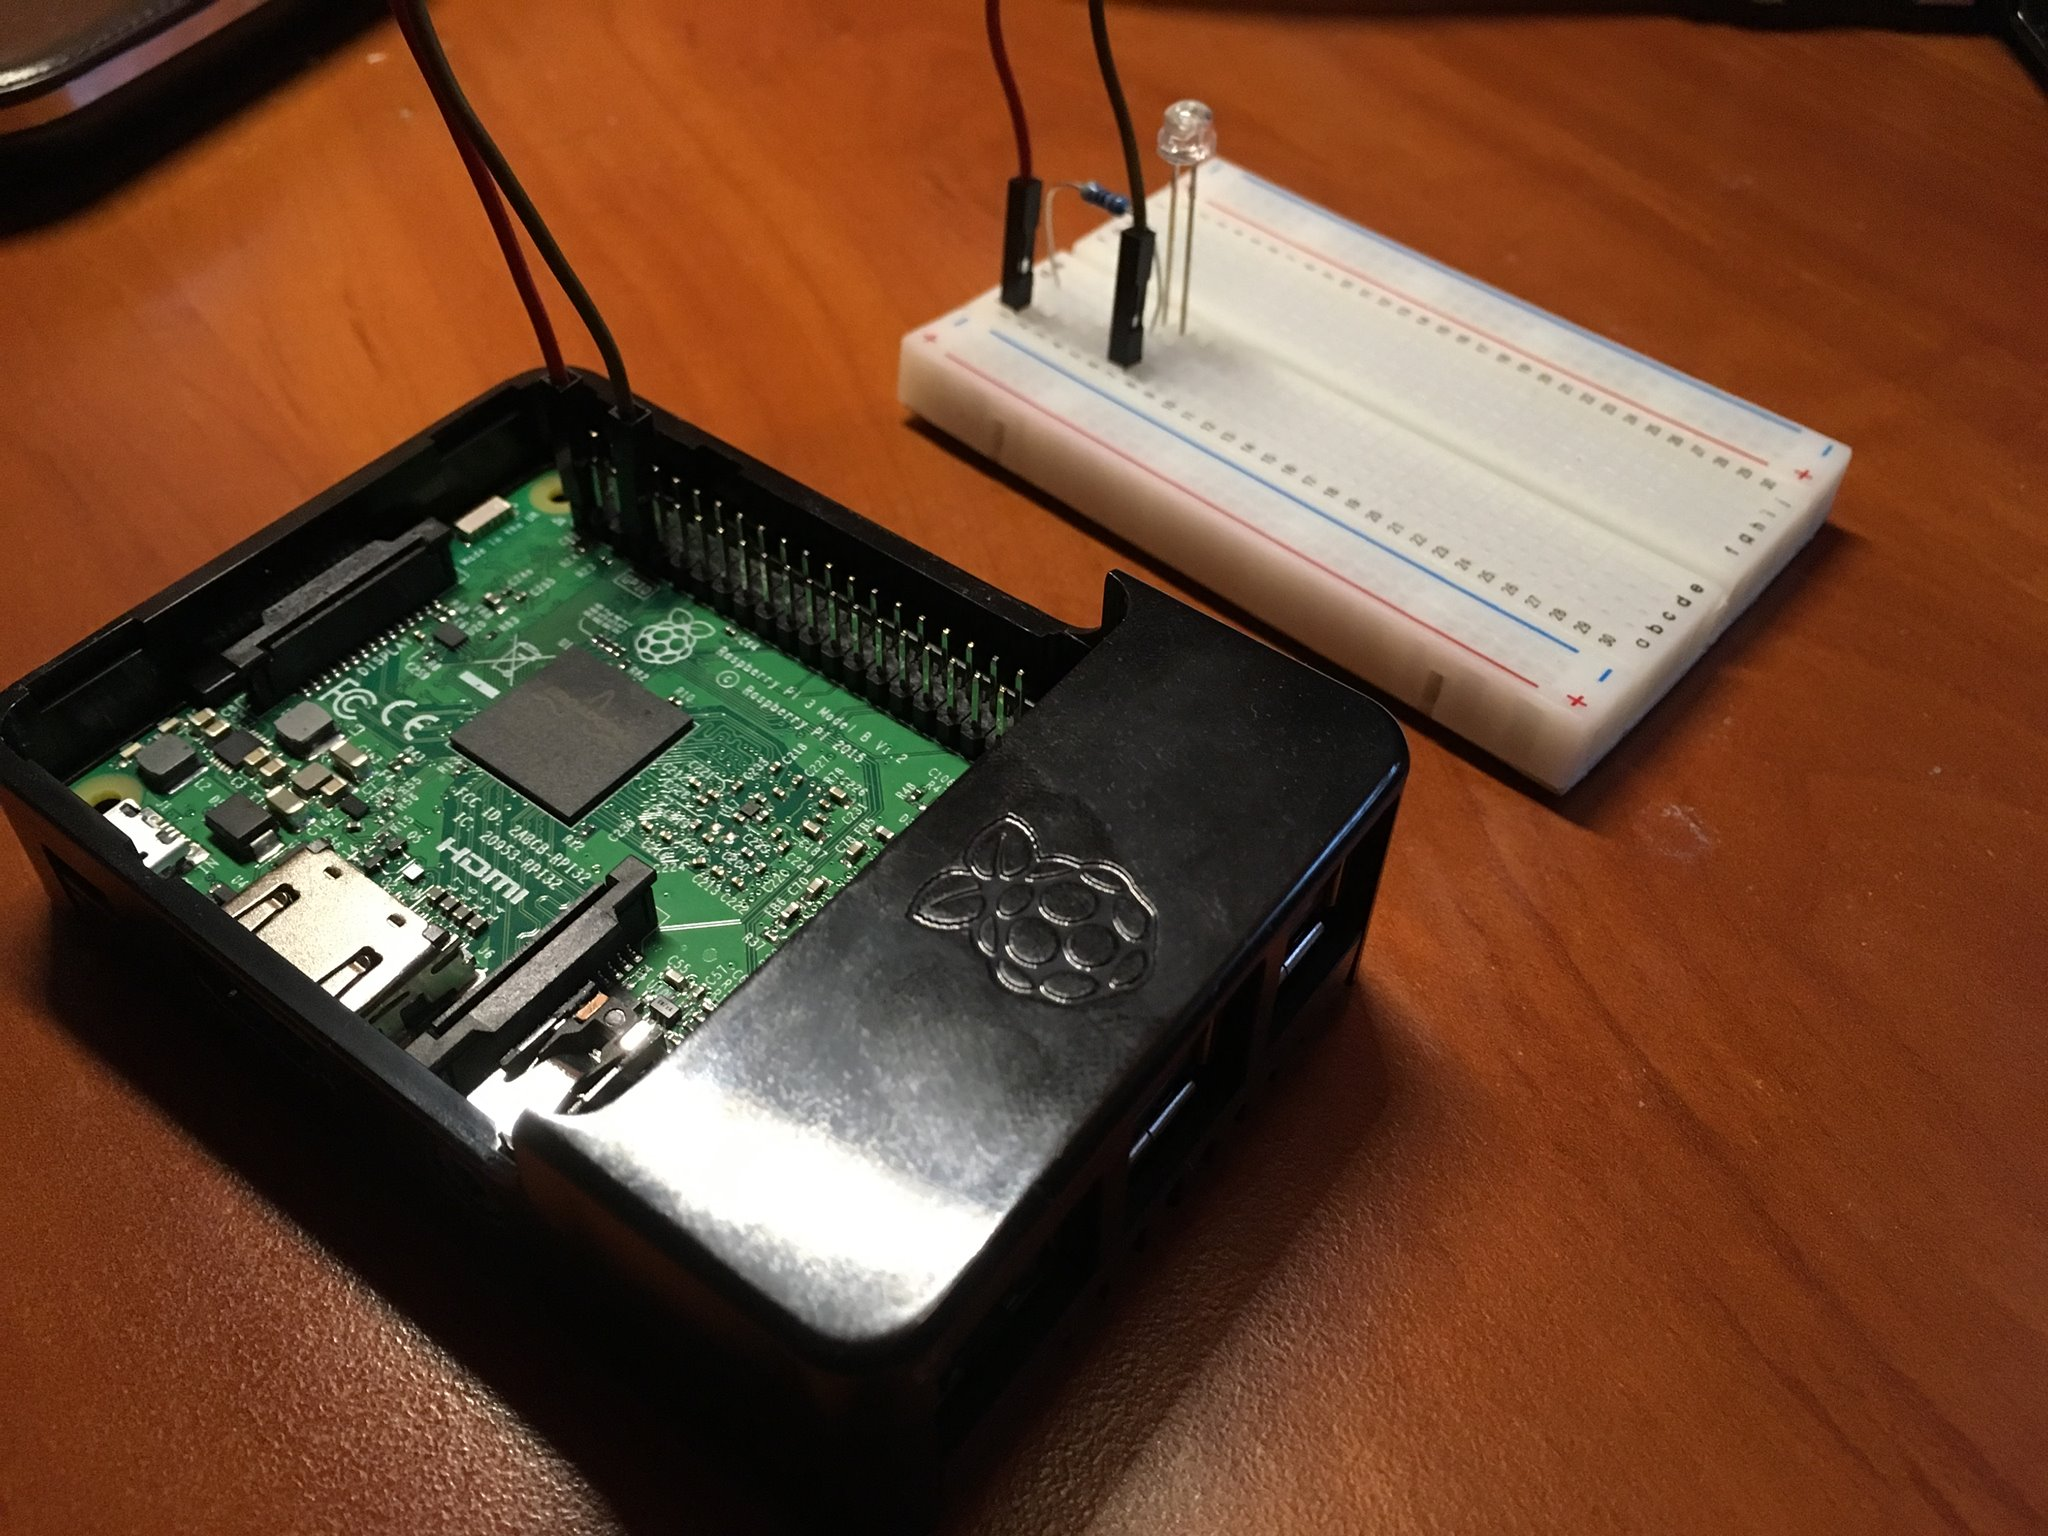
\includegraphics[width=\linewidth]{images/osszeszerelt3.jpg}
        \caption{Próbapanel rácsatlakoztatva a Raspberry Pi-re}
    \end{subfigure}
    \caption{Ha mindent jól csináltunk, a végeredmény így fog kinézni}
    \label{fig:összeszerelés}
\end{figure}

    A mikroprocesszorunk elkészült, most már alkalmas arra, hogy a IoT kliensalkalmazást futtassa.

\subsection{Telepítés}

\subsubsection{Asztali és mobilos környezetre}
    A felhasználói kliensalkalmazást a piactérről tudjuk letölteni, ha rákeresünk a ``KeepSwitched'' kulcsszóra. További
    teendőnk nincs, az érkező frissítéseket a program automatikusan letölteni és telepíti.
    A használathoz szükségünk van internet kapcsolatra és Facebook profilra.

\subsubsection{Raspberry Pi-re}
    Miután megfelelően összeszereltük a mikroprocesszorunkat, futtathatjuk az IoT kliensalkalmazást, melyet szintén a piactérről
    KeepSwitchedIoT néven tölthetünk le.
    Most következik az Application Deployment, tehát a letöltött alkalmazást futtatni fogjuk Raspberry Pi eszközünkön. Ezt
    megtehetjük böngészőből is, csak az Raspberry IP címére van szükségünk, amit leolvashatunk a képernyőről miután betöltött
    az eszköz.

\begin{figure}[h!]
    \hspace{5cm}
    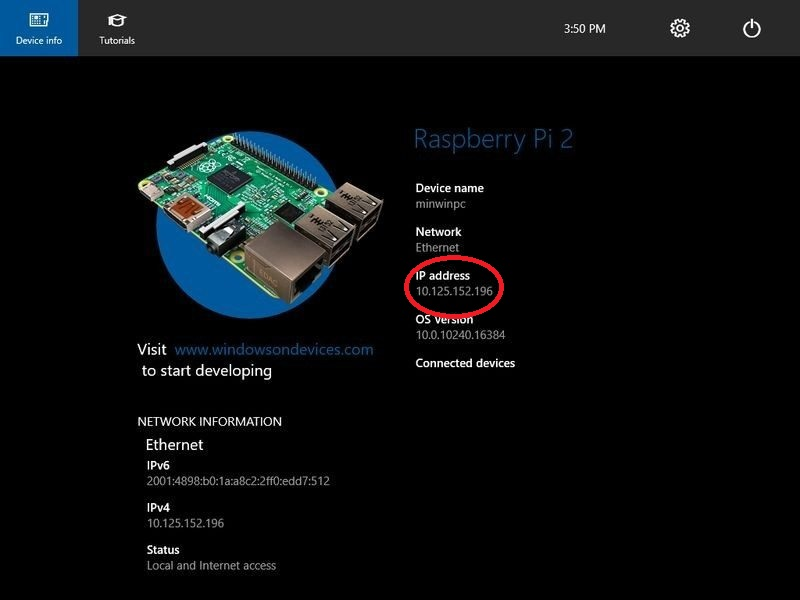
\includegraphics[width=6cm]{images/rpiip.jpg}
    \caption{A pirossal bekarikázott IP címre van szükségünk}
    \label{fig: Raspberry IP}
\end{figure}

    Másoljuk a kapott értéket a böngésző címsorába, és a \textbf{8080} - as porton keresztül tudjuk elérni eszközünket.
    Tehát ha az eszközünk IP címe például \textbf{192.168.0.105}, akkor az alábbi kerül a címsorba:

\begin{figure}[h!]
    \hspace{5cm}
    
\includegraphics[width=6cm]{images/browserrpi.jpg}
    \caption{A címsorba írandó IP cím}
    \label{fig: Raspberry IP Browser}
\end{figure}

    Ha helyen másoltuk ki az IP címet, akkor a böngésző kérni fog tőlünk egy felhasználónevet és jelszót. A Windows 10 IoT Core
    operációs rendszer esetén az alapértelmezett adatok az alábbiak:

\begin{itemize}
    \item Felhasználónév: ``\textbf{Administrator}''
    \item Jelszó: ``\textbf{p@ssw0rd}''
\end{itemize}

    Ha sikeres volt az authentikáció, akkor a Windows Device Portal felülete fog megjelenni előttünk, mely így fest:

\begin{figure}[h!]
    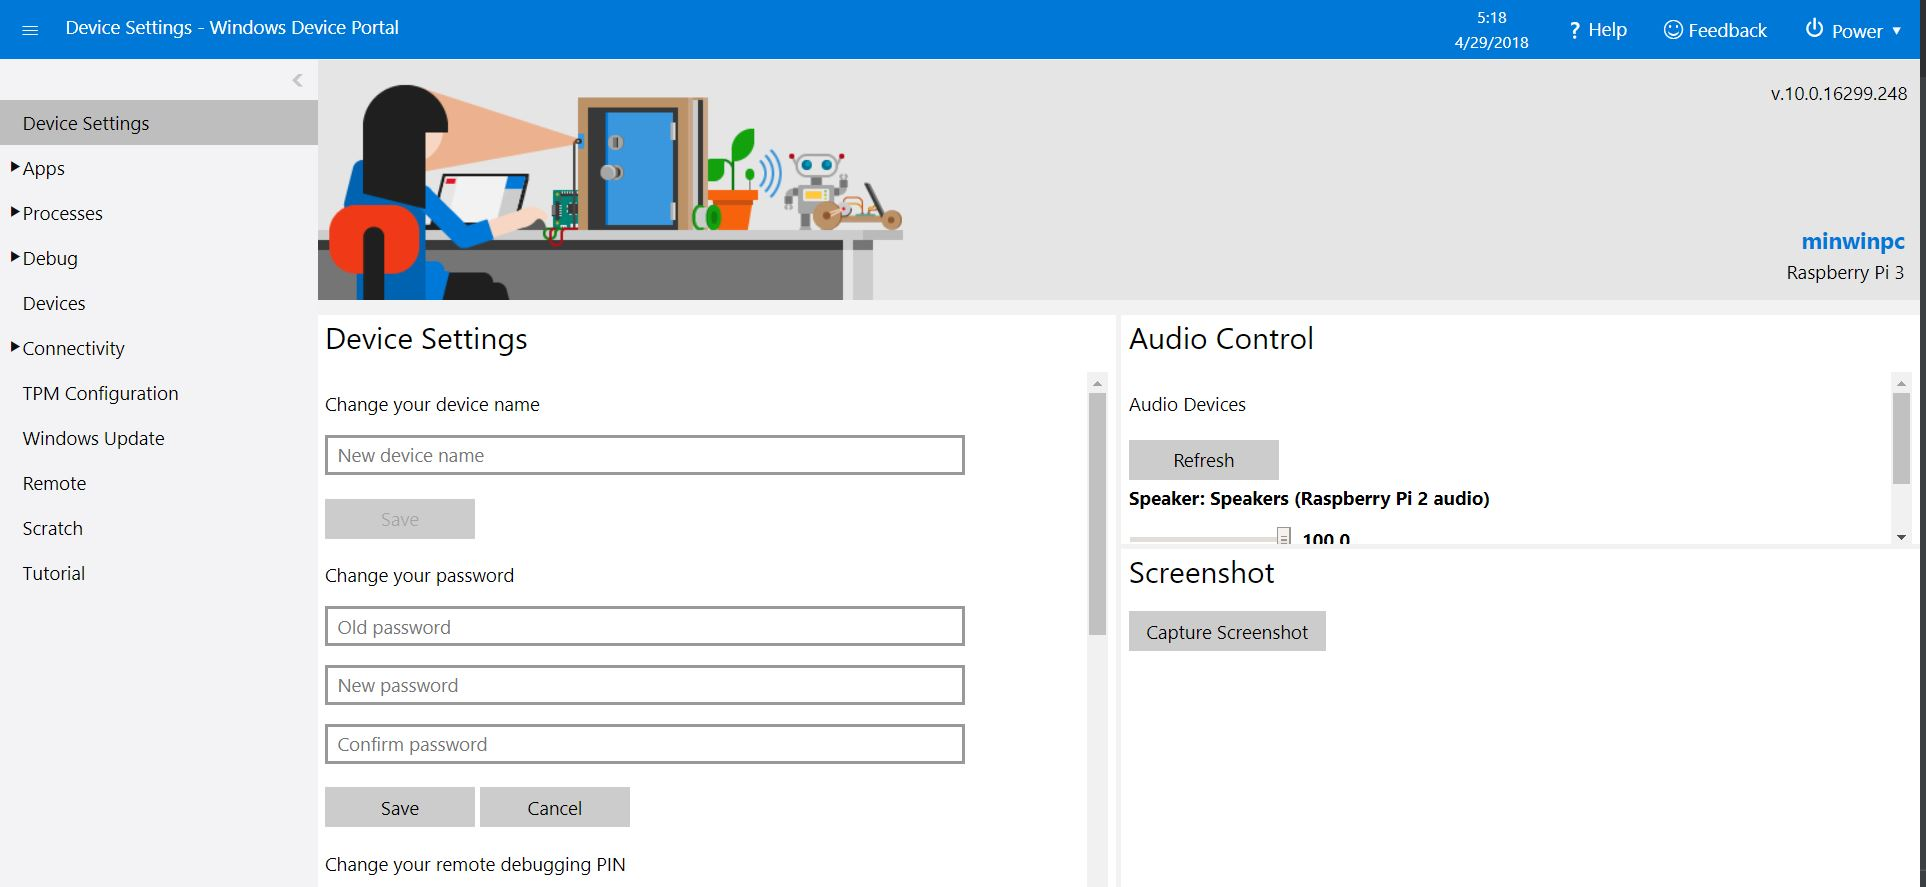
\includegraphics[width=\linewidth]{images/deviceportal.jpg}
    \caption{Windows Device Portal felülete}
    \label{fig: Windows Device Portal}
\end{figure}

    Ez egy nagyon hasznos felület, megváltoztathatjuk eszközünk nevét, jelszavát, felügyelhetjük a futó alkalmazásokat,
    kikapcsolhatjuk a Raspberry-t. De most egyelőre csak alkalmazást szeretnénk futtatni a mikroprocesszoron, így kattintsunk
    a bal oldalon található ``\textbf{Apps}"" fülre, majd az ``\textbf{Apps manager}"" lehetőségre.

\begin{figure}[h!]
    \centering
    \begin{subfigure}[b]{0.4\linewidth}
        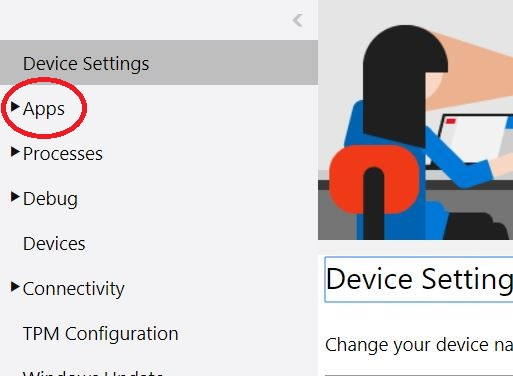
\includegraphics[width=\linewidth]{images/apps.jpg}
        \caption{Kattintsunk az Apps fülre}
    \end{subfigure}
    \begin{subfigure}[b]{0.4\linewidth}
        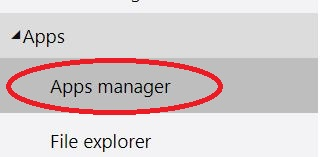
\includegraphics[width=\linewidth]{images/appsmanager.jpg}
        \caption{Majd az Apps Managerre}
    \end{subfigure}
    \caption{Navigáció alkalmazás hozzáadásához}
    \label{fig:Apps manager}
\end{figure}

    Most már majdnem készen vagyunk, válasszuk ki az ``\textbf{Add}'' lehetőséget, majd a megjelenő kis ablakban húzzuk bele
    a letöltött alkalmazást, vagy ki is kereshetjük a fájl böngészőből.

\begin{figure}[H]
    \centering
    \begin{subfigure}[b]{0.4\linewidth}
        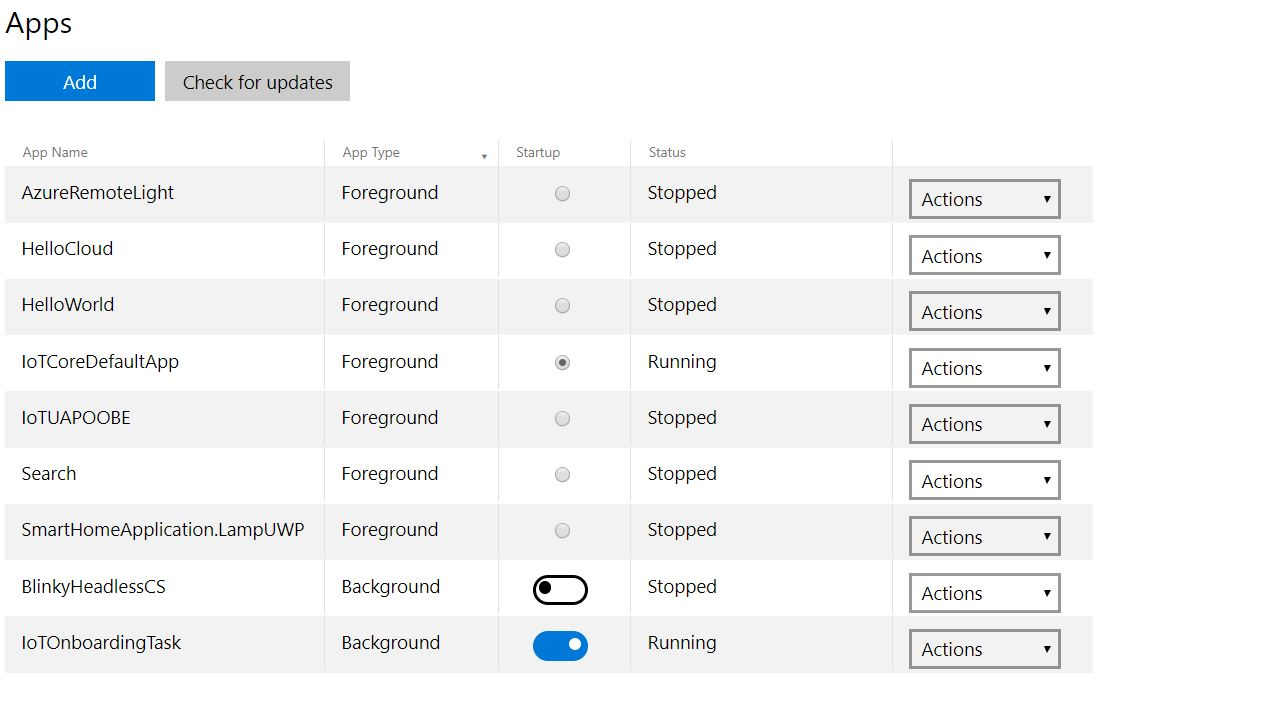
\includegraphics[width=\linewidth]{images/addapps.jpg}
        \caption{Kattinsunk az Add-ra}
    \end{subfigure}
    \begin{subfigure}[b]{0.4\linewidth}
        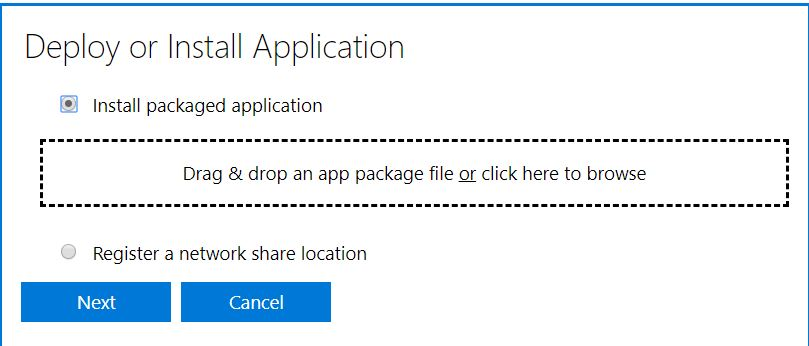
\includegraphics[width=\linewidth]{images/deploy.jpg}
        \caption{Húzzuk be, vagy keressük ki a letöltött alkalmazást}
    \end{subfigure}
    \caption{Alkalmazás hozzáadása}
    \label{fig:AddApps}
\end{figure}

    Ha mindent jól csináltunk, akkor a listában megjelenik alkalmazásunk és a mellette található legördülő menüben a ``\textbf{Start}''
    lehetőséget választva elindul az applikáció.

    \textbf{Fontos!} Áramszünet esetén a mikroprocesszor nem indítja el magától a programot, ehhez a ``\textbf{Startup}'' oszlopban
    be kell pipálnunk a lehetőséget.

\begin{figure}[h!]
    \centering
    \begin{subfigure}[b]{0.4\linewidth}
        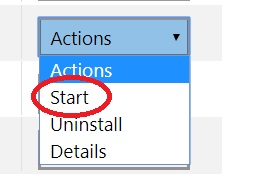
\includegraphics[width=\linewidth]{images/startapp.jpg}
        \caption{Indítsuk el az alkalmazást}
    \end{subfigure}
    \begin{subfigure}[b]{0.4\linewidth}
        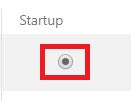
\includegraphics[width=\linewidth]{images/startupapp.jpg}
        \caption{Tegyük alapértelmezetté programunkat}
    \end{subfigure}
    \caption{Alkalmazás indítása és alapértelmezett futtatása}
    \label{fig:StartupApp}
\end{figure}
% ------------------------------------------------------------------------------



\end{document}
